\clearpage
\newgeometry{margin=1cm}
\thispagestyle{empty}
\begin{landscape}
\begin{table}[t!]
\caption[Key benchmark characteristics]{Key benchmark characteristics, using optimised source code}
\label{tbl-evaluation-benchmark-characteristics}
    \begin{tabular}{lrrrrrrrrrrrrrrr} % UPDATED 20180410
    \toprule
                                        & B.sort     &  H.sort    & Bin.Search & XXTEA      & MD5        & RC5        & FFT        & Outlier    & LEC        & CoreMark   & MoteTrack  & HeatCalib  & HeatDetect & \makebox[0.2mm]{} &   average \\
    \midrule
    \midrule
    \multicolumn{10}{l}{CODE SIZE (BYTES)} \\
    % Take JVM, Native C and AOT original from results_0BASE_R___P__C0_A0_S0_G1 (Java interpeter for JVM)
    \xxt Bytecode                       &         74 &        134 &         83 &        379 &       2983 &        453 &        441 &        287 &        334 &       2788 &       2552 &        310 &       2661 &                   &           \\
    \xxt Native C                       &        118 &        298 &        146 &       1442 &       9458 &        910 &       1292 &        380 &        560 &       6128 &       3906 &       1944 &       5294 &                   &           \\
    \xxt AOT original                   &        418 &       1012 &        412 &       3792 &      29502 &       4090 &       2576 &       1402 &       1628 &      13982 &      12784 &       2454 &      17248 &                   &           \\
    % Take AOT optimised from results_4MARK_R11_P7_C1_A1_S1_G1
    \xxt AOT optimised                  &        258 &        596 &        310 &       2236 &      14654 &       2018 &       1324 &        800 &       1056 &       8990 &       8478 &       1610 &      10346 &                   &           \\
    \midrule
    \multicolumn{10}{l}{EXECUTED BYTECODE INSTRUCTIONS (\% of total executed bytecode instructions before optimisation)} \\
    % Take this from results_0BASE_R___P__C0_A1_S0_G1 (16-bit array index enabled), otherwise we will get a lot of S2I conversions since the code uses shorts.
    \xxt Load/Store                     &       79.8 &       71.7 &       58.1 &       44.9 &       43.3 &       41.1 &       61.1 &       69.0 &       59.5 &       54.1 &       70.3 &       51.8 &       48.0 &                   &      57.9 \\
    \xxt Constant load                  &        0.2 &        8.1 &       11.0 &       12.5 &       19.1 &       17.6 &        6.4 &        0.6 &        7.9 &       10.0 &        5.4 &       10.1 &       16.6 &                   &       9.7 \\
    \xxt Processing                     &        8.0 &        7.8 &       14.8 &       32.4 &       28.9 &       36.6 &       18.0 &       13.0 &       12.7 &       14.0 &        5.9 &       17.9 &       10.3 &                   &      16.9 \\
      \xxxt   math                      & \xt    8.0 & \xt    5.5 & \xt   10.3 & \xt   10.1 & \xt   12.5 & \xt   10.7 & \xt   11.6 & \xt   13.0 & \xt    7.1 & \xt    8.2 & \xt    5.9 & \xt    3.7 & \xt    9.4 & \xt               & \xt   8.9 \\
      \xxxt   bit shift                 & \xt    0.0 & \xt    2.2 & \xt    4.5 & \xt    8.1 & \xt    5.4 & \xt    8.0 & \xt    6.1 & \xt    0.0 & \xt    3.8 & \xt    2.2 & \xt    0.0 & \xt    8.5 & \xt    0.9 & \xt               & \xt   3.8 \\
      \xxxt   bit logic                 & \xt    0.0 & \xt    0.0 & \xt    0.0 & \xt   14.2 & \xt   11.0 & \xt   17.9 & \xt    0.3 & \xt    0.0 & \xt    1.9 & \xt    3.6 & \xt    0.0 & \xt    5.7 & \xt    0.0 & \xt               & \xt   4.2 \\
    \xxt Branches                       &       12.0 &       10.9 &       15.5 &        4.0 &        5.8 &        2.3 &        5.1 &       17.4 &       10.5 &       16.0 &       13.6 &       14.7 &       19.2 &                   &      11.3 \\
    \xxt Invoke                         &        0.0 &        0.5 &        0.0 &        0.0 &        0.0 &        0.0 &        0.0 &        0.0 &        0.0 &        0.2 &        0.9 &        0.3 &        0.0 &                   &       0.1 \\
    \xxt Others                         &        0.0 &        1.0 &        0.6 &        0.2 &        2.5 &        2.4 &        9.4 &        0.0 &        7.1 &        4.7 &        2.2 &        4.2 &        5.9 &                   &       3.1 \\
    \xxt Total                          &      100.0 &      100.0 &      100.0 &      100.0 &      100.0 &      100.0 &      100.0 &      100.0 &      100.0 &      100.0 &      100.0 &      100.0 &      100.0 &                   &     100.0 \\
    \midrule
    % Take this from results_0BASE_R___P__C0_A1_S0_G1 as well.
    \multicolumn{10}{l}{STACK (bytes)} \\
    \xxt Max. stack                     &          6 &          8 &          4 &         24 &         20 &         14 &         10 &          6 &         18 &         16 &         12 &         22 &         16 &                   &      13.5 \\
    \xxt Avg. stack                     &       2.08 &       2.37 &       2.14 &      11.76 &       6.30 &       6.77 &       3.36 &       1.89 &       2.73 &       3.15 &       2.19 &       4.83 &       3.08 &                   &       4.1 \\
    \midrule
                                        & B.sort     &  H.sort    & Bin.Search & XXTEA      & MD5        & RC5        & FFT        & Outlier    & LEC        & CoreMark   & MoteTrack  & HeatCalib  & HeatDetect & \makebox[0.2mm]{} &   average \\
    \bottomrule
    \end{tabular}
\end{table}
\end{landscape}
\clearpage
\restoregeometry

\clearpage
\newgeometry{margin=1cm}
\thispagestyle{empty}
\begin{landscape}
\begin{table}[t!]
\caption{Performance data per benchmark}
\label{tbl-performance-per-benchmark}
    \begin{tabular}{lrrrrrrrrrrrrrrr} % UPDATED 20180410
    \toprule
                                        & B.sort     &  H.sort    & Bin.Search & XXTEA      & MD5        & RC5        & FFT        & Outlier    & LEC        & CoreMark   & MoteTrack  & HeatCalib  & HeatDetect & \makebox[0.2mm]{} &   average \\
    \midrule
    \midrule
    % Take this from performance-table.xlsx 
    \multicolumn{10}{l}{PERFORMANCE OVERHEAD USING ORIGINAL SOURCE (\% of native C)} \\
    \xxt Total                          &     1277.1 &     1927.2 &     1319.4 &      714.5 &      470.6 &      409.9 &      437.8 &      549.0 &      885.3 &      809.7 &     1018.7 &      210.2 &      203.9 &                   &     787.2 \\
      \xxxt push/pop                    & \xt  640.1 & \xt  356.7 & \xt  233.7 & \xt  197.2 & \xt  115.7 & \xt   70.1 & \xt   66.6 & \xt  207.2 & \xt  106.6 & \xt  220.4 & \xt  166.5 & \xt   80.9 & \xt   78.8 & \xt               & \xt 195.4 \\
      \xxxt load/store                  & \xt  360.1 & \xt  197.4 & \xt  175.3 & \xt   67.0 & \xt   46.7 & \xt   33.2 & \xt   29.3 & \xt  190.3 & \xt  110.7 & \xt  136.8 & \xt  218.2 & \xt   67.6 & \xt   43.8 & \xt               & \xt 129.0 \\
      \xxxt mov(w)                      & \xt   10.0 & \xt   41.1 & \xt    8.4 & \xt    6.6 & \xt    3.6 & \xt    0.1 & \xt    5.2 & \xt   21.5 & \xt    5.1 & \xt    5.5 & \xt   38.6 & \xt   -3.0 & \xt    9.5 & \xt               & \xt  11.7 \\
      \xxxt other                       & \xt  266.9 & \xt  331.4 & \xt  902.1 & \xt   82.8 & \xt  104.0 & \xt   67.8 & \xt   76.8 & \xt  130.1 & \xt  370.6 & \xt  234.2 & \xt  220.0 & \xt   37.4 & \xt   65.6 & \xt               & \xt 222.3 \\
      \xxxt vm                          & \xt    0.0 & \xt 1000.6 & \xt    0.0 & \xt  361.1 & \xt  200.4 & \xt  238.7 & \xt  260.0 & \xt   -0.1 & \xt  292.2 & \xt  212.9 & \xt  375.4 & \xt   27.3 & \xt    6.2 & \xt               & \xt 228.8 \\
    \multicolumn{10}{l}{OVERHEAD REDUCTION FROM SOURCE CODE OPTIMISATION (\% of native C)} \\
    \xxt Source optimisation            &     -613.2 &    -1234.0 &     -843.6 &     -464.1 &     -244.2 &     -285.6 &     -315.0 &      -56.5 &     -612.7 &     -433.7 &     -227.9 &        0.0 &        1.7 &                   &    -409.9 \\
    \midrule
    \multicolumn{10}{l}{PERFORMANCE OVERHEAD BEFORE COMPILER OPTIMISATIONS (\% of native C)} \\
    \xxt Total                          &      663.9 &      693.2 &      475.8 &      250.4 &      226.4 &      124.3 &      122.8 &      492.5 &      272.6 &      376.0 &      790.8 &      210.2 &      205.6 &                   &     377.3 \\
      \xxxt push/pop                    & \xt  266.9 & \xt  200.8 & \xt  202.2 & \xt  166.4 & \xt  105.3 & \xt   61.9 & \xt   57.2 & \xt  205.5 & \xt  105.6 & \xt  123.8 & \xt  137.7 & \xt   80.9 & \xt   77.5 & \xt               & \xt 137.8 \\
      \xxxt load/store                  & \xt  240.3 & \xt  177.5 & \xt  191.0 & \xt   42.5 & \xt   43.9 & \xt   28.5 & \xt   25.2 & \xt  190.4 & \xt  111.7 & \xt   89.2 & \xt  165.3 & \xt   67.6 & \xt   47.6 & \xt               & \xt 109.3 \\
      \xxxt mov(w)                      & \xt   23.3 & \xt   14.8 & \xt    4.5 & \xt    3.9 & \xt    2.6 & \xt   -1.2 & \xt    4.2 & \xt    8.0 & \xt    5.1 & \xt    5.3 & \xt   17.6 & \xt   -3.0 & \xt   10.9 & \xt               & \xt   7.4 \\
      \xxxt other                       & \xt  133.5 & \xt  118.4 & \xt   78.1 & \xt   37.7 & \xt   74.6 & \xt   35.1 & \xt   36.2 & \xt   88.8 & \xt   49.0 & \xt   97.7 & \xt   94.8 & \xt   37.4 & \xt   63.4 & \xt               & \xt  72.7 \\
      \xxxt vm                          & \xt    0.0 & \xt  181.7 & \xt    0.0 & \xt    0.0 & \xt    0.0 & \xt    0.0 & \xt    0.0 & \xt   -0.1 & \xt    1.1 & \xt   60.0 & \xt  375.4 & \xt   27.3 & \xt    6.2 & \xt               & \xt  50.1 \\
    \multicolumn{10}{l}{OVERHEAD REDUCTION PER COMPILER OPTIMISATION (\% of native C)} \\
    \xxt Impr. peephole                 &     -233.5 &     -157.7 &     -149.4 &      -60.3 &      -48.2 &      -23.1 &      -36.5 &     -186.9 &      -54.2 &      -58.8 &      -60.2 &      -35.2 &      -54.5 &                   &     -89.1 \\
    \xxt Stack caching                  &      -40.0 &      -56.0 &      -57.3 &      -98.4 &      -58.0 &      -39.8 &      -16.2 &      -27.8 &      -67.7 &      -40.7 &      -63.1 &      -41.4 &      -24.2 &                   &     -48.6 \\
    \xxt Pop. val. caching              &     -133.1 &      -84.9 &      -67.4 &       -6.8 &      -12.9 &       -8.8 &      -10.7 &      -51.0 &      -28.8 &      -24.5 &      -41.5 &      -15.4 &      -15.5 &                   &     -38.5 \\
    \xxt Mark loops                     &     -102.9 &      -46.8 &      -85.4 &       +5.0 &      -10.9 &       -8.0 &       -7.9 &     -114.9 &      -18.0 &      -40.0 &      -54.3 &      -38.2 &      -28.6 &                   &     -42.4 \\
    \xxt Const shift                    &        0.0 &      -17.1 &      -35.4 &      -18.4 &      -45.2 &      -20.9 &       -3.8 &        0.0 &       -9.6 &      -10.1 &        0.0 &      -17.2 &       -3.3 &                   &     -13.9 \\
    \xxt 16-bit array index             &      -53.2 &      -34.9 &      -15.7 &      -13.9 &       -5.5 &       -4.2 &       -2.8 &      -36.2 &       -9.7 &      -38.9 &      -19.7 &       -1.7 &       -9.0 &                   &     -18.9 \\
    \xxt SIMUL                          &        0.0 &        0.0 &        0.0 &        0.0 &        0.0 &        0.0 &      -27.2 &        0.0 &        0.0 &      -36.6 &        0.0 &        0.0 &        0.0 &                   &      -4.9 \\
    \xxt Lightw. methods                &        0.0 &     -207.3 &        0.0 &        0.0 &        0.0 &        0.0 &        0.0 &        0.0 &        0.0 &      -67.5 &     -395.7 &      -30.6 &       -0.3 &                   &     -54.0 \\
    \multicolumn{10}{l}{PERFORMANCE OVERHEAD AFTER COMPILER OPTIMISATIONS (\% of native C)} \\
    \xxt Total                          &      101.2 &       88.5 &       65.2 &       57.6 &       45.7 &       19.5 &       17.7 &       75.7 &       84.6 &       58.9 &      156.3 &       30.5 &       70.2 &                   &      67.0 \\
      \xxxt push/pop                    & \xt    0.0 & \xt   -2.8 & \xt    0.0 & \xt   37.4 & \xt    0.1 & \xt    2.9 & \xt    2.0 & \xt   -0.2 & \xt  -13.7 & \xt    2.5 & \xt   20.4 & \xt    5.6 & \xt    1.7 & \xt               & \xt   4.3 \\
      \xxxt load/store                  & \xt    1.0 & \xt   29.3 & \xt   27.0 & \xt   -2.3 & \xt   20.3 & \xt    4.3 & \xt    2.4 & \xt    4.5 & \xt   54.3 & \xt   17.1 & \xt   72.0 & \xt    2.7 & \xt   13.5 & \xt               & \xt  18.9 \\
      \xxxt mov(w)                      & \xt   10.0 & \xt    9.4 & \xt   11.8 & \xt    5.6 & \xt    1.5 & \xt    0.1 & \xt    2.9 & \xt    6.8 & \xt    7.4 & \xt    9.6 & \xt   14.9 & \xt    5.1 & \xt    4.4 & \xt               & \xt   6.9 \\
      \xxxt other                       & \xt   90.2 & \xt   52.5 & \xt   26.4 & \xt   16.9 & \xt   23.8 & \xt   12.2 & \xt   10.4 & \xt   64.7 & \xt   35.5 & \xt   28.8 & \xt   35.7 & \xt   17.0 & \xt   46.1 & \xt               & \xt  35.4 \\
      \xxxt vm                          & \xt    0.0 & \xt    0.0 & \xt    0.0 & \xt    0.0 & \xt    0.0 & \xt    0.0 & \xt    0.0 & \xt   -0.1 & \xt    1.1 & \xt    0.8 & \xt   13.2 & \xt    0.0 & \xt    4.4 & \xt               & \xt   1.5 \\
    \midrule
                                        & B.sort     &  H.sort    & Bin.Search & XXTEA      & MD5        & RC5        & FFT        & Outlier    & LEC        & CoreMark   & MoteTrack  & HeatCalib  & HeatDetect & \makebox[0.2mm]{} &   average \\
    \bottomrule
    \end{tabular}
\end{table}
\end{landscape}
\clearpage
\restoregeometry



\section{AOT translation: performance}
\label{sec-evaluation-aot-translation-performance}

Next we will look at the effect of our optimisations to the baseline AOT translation approach, for all our benchmarks.

The trace data produced by Avrora gives us a detailed view into the run-time performance and the different types of overhead. We count the number of bytes and cycles spent on each native instruction for both the native C and our AOT compiled version, and group them into 4 categories that roughly match the types of AOT translation overhead discussed in Section \ref{sec-overhead-aot-translation}:
\begin{itemize}
	\item \mycode{PUSH},\mycode{POP}: Matches the type 1 push/pop overhead since native code uses almost no push/pop instructions.
	\item \mycode{LD},\mycode{LDD},\mycode{ST},\mycode{STD}: Matches the type 2 load/store overhead and directly shows the amount of memory traffic.
	\item \mycode{MOV},\mycode{MOVW}: For moves the picture is less clear since the AOT compiler emits them for various reasons. Without stack caching, it emits moves to replace push/pop pairs, and after adding the mark loops optimisation to save a pinned value when it is popped destructively.
	\item others: the total overhead, minus the previous three categories. This roughly matches the type 3 overhead.
\end{itemize}

We define the overhead from each category as the number of bytes or cycles spent in the AOT version, minus the number spent in the native version for that category, and again normalise this to the \emph{total} number of bytes or cycles spent in the native C version. The detailed results for each benchmark and type of overhead are shown in tables \ref{tbl-performance-per-benchmark} and \ref{tbl-codesize-per-benchmark}. In addition, Table \ref{tbl-performance-per-benchmark} also lists the time spent in the VM on method calls and allocating objects. The constant array optimisation is already included in these results, since MoteTrack cannot run without it. We will examine its effect separately in section \ref{sec-evaluation-const-array}.

The baseline shown in Table \ref{tbl-performance-per-benchmark} before optimisation is the original, direct translation of the C code to Java. This results in a large overhead of up to 20x slowdown for \mybench{heap sort}, most of which is due to method calls since small functions and macros in the C code are not inlined in this version. Optimising the source code reduces overhead dramatically, but this is partly because the other optimisations, which target some of the same overhead, have not yet been applied. For example, in Table \ref{tbl-performance-per-benchmark} optimising the source code reduces \mybench{CoreMark}'s overhead by 434\%, while the previous section showed that when all other optimisations are applied first, the difference is only 268\%. Since the source code optimisations were discussed in the previous section, the rest of this evaluation will focus on the effect of the other optimisations on the already optimised source.

Figure \ref{fig-performance-per-opcode-category} starts with the manually optimised source code and incrementally adds each optimisation to the AOT compilation process to show how they combine to reduce performance overhead. We take the average of all benchmarks, and show both the total overhead, and the overhead for each instruction category. Figure \ref{fig-performance-per-benchmark} shows the total overhead for each individual benchmark.

\begin{figure}
\centering
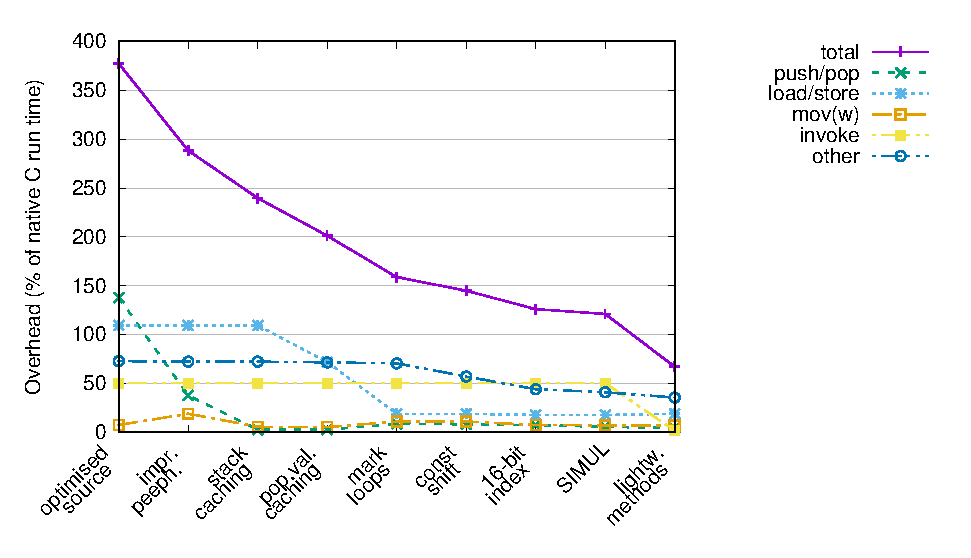
\includegraphics[width=\mygraphsize]{performance-per-opcode-category3a.eps}
\caption{Performance overhead per category}
\label{fig-performance-per-opcode-category}
\end{figure}

\begin{figure}
\centering
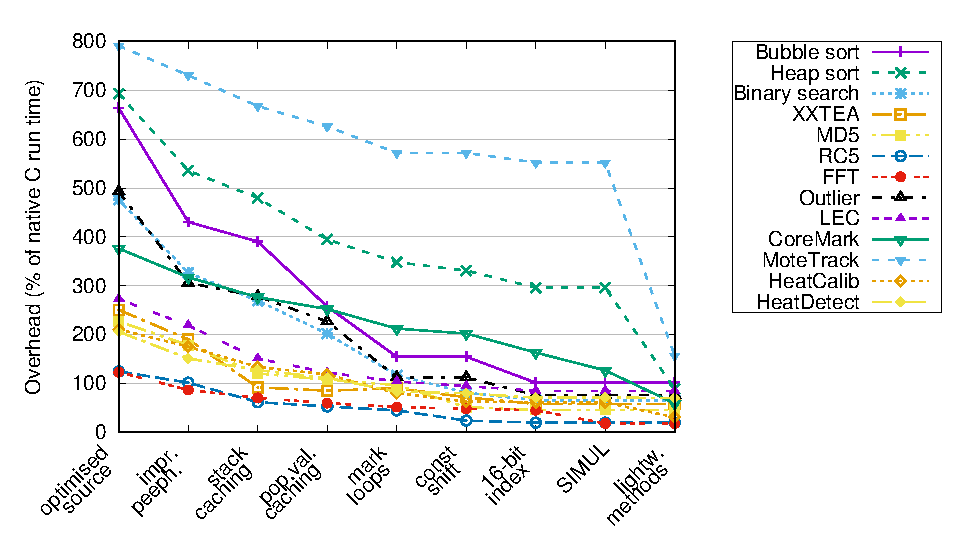
\includegraphics[width=\mygraphsize]{performance-per-benchmark3a.eps}
\caption{Performance overhead per benchmark}
\label{fig-performance-per-benchmark}
\end{figure}

Using the baseline AOT compilation on the optimised sources, the types 1, 2 and 3 overhead are all significant, at 138\%,  109\%, and 73\% respectively, and the 50\% overhead in the VM is mainly spent on method calls since the overhead from allocating temporary objects is removed by the source code optimisations. The basic approach does not have many reasons to emit a move, so in some cases the AOT version actually spends fewer cycles on move instructions than the C version, resulting in small negative values.  When we improve the peephole optimiser to include non-consecutive push/pop pairs, push/pop overhead drops by 100.2\% (of native C performance), but if the push and pop target different registers, they are replaced by a move instruction, and we see an increase of 11.5\% in move overhead. For a 16-bit register pair this takes 1 cycle (for a \mycode{MOVW} instruction), instead of 8 cycles for two pushes and two pops. The increase in moves shows most of the extra cases that are handled by the improved optimiser are replaced by a move instead of eliminated, since the 11.5\% extra move overhead matches a 92\% reduction in push/pop overhead.

Next stack caching is introduced to utilise all available registers and eliminate most of the push/pop instructions that cannot be handled by the improved optimiser. As a result the push/pop overhead drops to nearly 0, and so does the move overhead since most of the moves introduced by the peephole optimiser, are also unnecessary when using stack caching.

Having eliminated the type 1 overhead almost completely, popped value caching is added to remove a large number of the unnecessary load instructions. This reduces the memory traffic significantly, as is clear from the reduced load/store overhead, while the other types remain stable. Adding the mark loops optimisation further reduces loads, and this time also stores, by pinning common variables to a register. But it uses slightly more move instructions, and the fact that fewer registers are available for stack caching means stack values are spilled to memory more often. While 53.0\% is saved on loads and stores, the push/pop and move overhead increase by 6.0\% and 5.6\% respectively.

Most of the push/pop and load/store overhead has now been eliminated and the type 3 overhead, unaffected by these optimisations, has become the most significant source of overhead. This type has many different causes, part of it can be eliminated with the instruction set optimisations. These optimisations, especially the 16-bit array index, also reduce register pressure, which results in a slight decrease in the other overhead types, although this is minimal in comparison. The \mybench{CoreMark} and \mybench{FFT} benchmarks are the only ones to do 16-bit to 32-bit multiplication, so the average performance improvement for \mycode{SIMUL} is small, but Table \ref{tbl-performance-per-benchmark} shows it is significant for these two benchmarks.

Finally, the lightweight optimisation could be applied to almost every method. Lightweight methods still incur some overhead, which will be discussed in more detail in Section \ref{sec-evaluation-method-invocation}, but since they do not call the VM, the time spent in the VM on method calls is effectively eliminated.

Combined, the optimisations to the AOT compilation process reduce performance overhead from 377\% to 67\% of native C performance.
